\chapter{Optimal Transport の基礎理論}
\label{ch:seminar-01}

\begin{remark}{本章の設定}{sem-ch2-setup}
  $(\X, d_\X)$, $(\Y, d_\Y)$ は\textbf{完備可分な距離空間}（Polish 空間，
  定義~\ref{def:sem-polish}）とする．
  ボレル $\sigma$-代数 $\Bb(\X)$ により $\X$ を可測空間 $(\X, \Bb(\X))$ として扱う
  （$\Y$ についても同様）．$\X$ 上の確率測度全体を $\Mm_+^1(\X)$ と記す．

  Polish 空間の3要素を確認する：
  \begin{itemize}
    \item \textbf{距離空間}．距離関数
      $d_\X \colon \X \times \X \to [0, \infty)$ が距離の公理
      （定義~\ref{def:sem-metric-space}）を満たし，$d_\X$ から以下が順次定まる：
      \begin{align*}
        B_r(x)
          &\defeq \{y \in \X \mid d_\X(x, y) < r\}
          && \text{（開球，定義~\ref{def:sem-open-ball}）} \\
        \mathcal{O}_{d_\X}
          &\defeq \{U \subset \X \mid \forall x \in U,\,
            \exists r > 0,\, B_r(x) \subset U\}
          && \text{（開集合の全体）} \\
        \Bb(\X)
          &\defeq \sigma(\mathcal{O}_{d_\X})
          && \text{（ボレル } \sigma\text{-代数，定義~\ref{def:sem-borel}）}
      \end{align*}
      ここで $\sigma(\mathcal{O}_{d_\X})$ は，$\mathcal{O}_{d_\X}$ を含む
      $\X$ 上のすべての $\sigma$-代数の共通部分
      \[
        \sigma(\mathcal{O}_{d_\X})
        \defeq \bigcap
        \bigl\{
          \mathcal{F} \subset 2^{\X}
          \;\big|\;
          \mathcal{F} \text{ は } \sigma\text{-代数, }
          \mathcal{O}_{d_\X} \subset \mathcal{F}
        \bigr\}
      \]
      として定まる．これにより可測空間 $(\X, \Bb(\X))$
      （定義~\ref{def:sem-measurable-space}）が得られる．
    \item \textbf{完備性}．
      列 $(x_n)_{n \geq 1} \subset \X$ が\textbf{Cauchy 列}であるとは，
      任意の $\varepsilon > 0$ に対してある $N \in \N$ が存在して
      $n, m \geq N \Longrightarrow d_\X(x_n, x_m) < \varepsilon$ が成り立つことをいう．
      $(\X, d_\X)$ が完備とは，任意の Cauchy 列 $(x_n) \subset \X$ が
      $\X$ の点に収束する（定義~\ref{def:sem-convergence}）ことをいう．
      すなわち
      \[
        \forall (x_n) \subset \X \text{ Cauchy 列},\;
        \exists x \in \X,\; x_n \to x.
      \]
      収束の定義に展開すれば
      \[
        \forall (x_n) \subset \X \text{ Cauchy 列},\;
        \exists x \in \X,\;
        \forall \varepsilon > 0,\;
        \exists N \in \N,\;
        n \geq N \Longrightarrow d_\X(x_n, x) < \varepsilon.
      \]
    \item \textbf{可分性}．
      $D \subset \X$ が\textbf{稠密}であるとは，任意の空でない開集合
      $U \subset \X$ に対し $D \cap U \neq \emptyset$ となることをいう
      （定義~\ref{def:sem-dense}）．
      距離空間ではこれは「任意の $x \in \X$ と任意の $\varepsilon > 0$ に対し
      $\exists q \in D,\; d_\X(x, q) < \varepsilon$」と同値．
      $(\X, d_\X)$ が可分とは可算な稠密部分集合 $D \subset \X$ が
      存在することをいう（定義~\ref{def:sem-separable}）．すなわち
      \[
        \exists D \subset \X \text{ 可算},\;
        \forall U \subset \X \text{ 空でない開集合},\;
        D \cap U \neq \emptyset.
      \]
  \end{itemize}

  離散版では確率測度の表示に現れる点集合
  $S \defeq \{x_1, \ldots, x_n\} \subset \X$ は有限集合となる．
  $S$ にどの距離 $d$ を入れた距離空間 $(S, d)$ も
  自動で Polish 空間となる（$\X$ の可測構造は $S$ に制限することで継承される）：
  \begin{itemize}
    \item[] \textbf{完備性．} $n = 1$ なら $S = \{x_1\}$ ゆえ
      任意の列は $y_k = x_1$ ($\forall k$) なる定値列であり，
      $d(y_k, x_1) = 0$ より $x_1$ に収束する．
      以下 $n \geq 2$ とする．相異なる 2 点間の距離の最小値を
      $\delta \defeq \min_{i \neq j} d(x_i, x_j)$ とおく．
      これは有限個の正数の最小値なので $\delta > 0$．
      任意の Cauchy 列 $(y_k)_{k \geq 1} \subset S$ に対し，
      Cauchy 条件で $\varepsilon \defeq \delta / 2$ を取ると，
      ある $N \in \N$ が存在して
      $k, l \geq N \Longrightarrow d(y_k, y_l) < \delta / 2 < \delta$．
      一方 $S$ の相異なる 2 点の距離は $\delta$ 以上だから，
      $d(y_k, y_l) < \delta$ は $y_k = y_l$ を強制する．
      ゆえに列 $(y_k)$ は $N$ 以降すべて同一の点となり，その点に収束する．
    \item[] \textbf{可分性．} $S$ 自身が有限（特に可算）集合であり，
      自身の中で稠密だから可分．
  \end{itemize}
  したがって本章の Polish 強化は連続側で必要となる一方，
  離散版には追加制約を課さない．
\end{remark}

%% ============================================================
%% 最適割当問題（§2.2 前半）
%% ============================================================
\section{最適割当問題}
\label{sec:sem-assignment}

\begin{definition}{最適割当問題}{sem-assignment}
  $n \in \N$，置換 $\sigma \in \Perm(n)$，
  および行列 $\mathbf{C} \in \R_+^{n \times n}$ に対して，
  \[
    \min_{\sigma \in \Perm(n)} \frac{1}{n} \sum_{i=1}^{n} C_{i, \sigma(i)}
  \]
  を達成する $\sigma$ を求める問題を\textbf{最適割当問題}という．
\end{definition}

添字 $i$ から $j$ への\textbf{輸送コスト}を $C_{i,j}$ と解釈すれば，
$\sigma(i) = j$ は $i$ を $j$ に割り当てることを意味し，
目的関数 $\frac{1}{n}\sum_i C_{i, \sigma(i)}$ はその割当の平均輸送コストを表す．

\begin{example}{最適割当}{sem-assignment-cost-example}
  $n = 2$ とし，置換 $\sigma \in \Perm(2)$ と行列
  \[
    \mathbf{C} =
    \begin{pmatrix}
      1 & 4 \\
      2 & 1
    \end{pmatrix} \in \R_+^{2 \times 2}
  \]
  を考える．$\Perm(2) = \{(1,2),\, (2,1)\}$ の $2! = 2$ 通りの割当を以下に図示する．

  \begin{center}
  \begin{tikzpicture}[
    wk/.style={circle, draw=blue!60, fill=blue!10,
               minimum size=18pt, inner sep=1pt, font=\small},
    tk/.style={rectangle, rounded corners=1.5pt,
               draw=red!60, fill=red!10,
               minimum size=18pt, inner sep=1pt, font=\small},
    optarr/.style={-{Stealth[length=5pt]}, thick, green!50!black},
    arr/.style={-{Stealth[length=5pt]}, semithick, black!60, dashed},
    costlbl/.style={fill=white, inner sep=1pt, font=\footnotesize},
  ]
    \node[wk] (w1) at (0, 1.2) {1};
    \node[wk] (w2) at (3, 1.2) {2};
    \node[tk] (t1) at (1, -1.2) {1};
    \node[tk] (t2) at (4, -1.2) {2};

    % σ=(1,2): 1→1, 2→2（最適）
    \draw[optarr] (w1) -- node[costlbl, midway] {(a)\ $1$} (t1);
    \draw[optarr] (w2) -- node[costlbl, midway] {(a)\ $1$} (t2);
    % σ=(2,1): 1→2, 2→1
    \draw[arr] (w1) -- node[costlbl, pos=0.25] {(b)\ $4$} (t2);
    \draw[arr] (w2) -- node[costlbl, pos=0.25] {(b)\ $2$} (t1);
  \end{tikzpicture}
  \end{center}

  各割当のコストをまとめると，
  \begin{center}
  \begin{tabular}{ccc}
     & $\sigma$ & コスト $\frac{1}{n}\sum_i C_{i,\sigma(i)}$ \\\hline
    (a) & $(1,2)$ & $\frac{1}{2}(1 + 1) = \mathbf{1}$ \\
    (b) & $(2,1)$ & $\frac{1}{2}(4 + 2) = 3$ \\
  \end{tabular}
  \end{center}
  よって $\sigma = (1, 2)$ が最小コスト $1$ を達成し，最適である．
\end{example}

\begin{claim}{最適解の存在}{sem-assignment-existence}
  任意の $n \in \N$ と任意の $\mathbf{C} \in \R_+^{n \times n}$ に対して，
  最適割当問題の最小値は達成される．
\end{claim}

\begin{proof}
  $\Perm(n)$ は $|\Perm(n)| = n!$ の有限集合なので，集合
  \[
    \left\{ \frac{1}{n}\sum_{i=1}^{n} C_{i, \sigma(i)} \;\middle|\; \sigma \in \Perm(n) \right\}
  \]
  は高々 $n!$ 個の実数からなる空でない有限集合である．
  $\R$ の空でない有限部分集合は最小元を持つ（主張~\ref{clm:sem-finite-min}）
  ので，それを達成する $\sigma^* \in \Perm(n)$ が存在する．
\end{proof}

\begin{claim}{最適解が一意でない場合の存在}{sem-uniqueness}
  任意の $n \geq 2$ に対して，
  異なる $\sigma_1, \sigma_2 \in \Perm(n)$ がともに最小値を達成するような
  $\mathbf{C} \in \R_+^{n \times n}$ が存在する．
\end{claim}

\begin{proof}
  $C_{i,j} \defeq 1$（$i, j = 1, \ldots, n$）と定めると，任意の $\sigma \in \Perm(n)$ に対して
  $\frac{1}{n}\sum_{i=1}^{n} C_{i, \sigma(i)} = 1$．
  異なる $\sigma_1, \sigma_2 \in \Perm(n)$ を取れば，
  いずれも最小値 $1$ を達成する．
\end{proof}

%% ============================================================
%% Monge 問題（§2.2 後半）
%% ============================================================
\section{Monge 問題}
\label{sec:sem-monge}

最適割当問題（定義~\ref{def:sem-assignment}）は有限の添字集合 $\range{n}$ と
均一重み $1/n$ を扱う離散的な輸送問題だった．次の対応で一般の Polish 空間
$\X, \Y$ と任意の確率測度に拡張する：
\begin{center}
  \begin{tabular}{l|ll}
    & 最適割当問題 & Monge 問題 \\ \hline
    source/target & $\range{n}$（重み $1/n$） & $\alpha \in \Mm_+^1(\X)$，$\beta \in \Mm_+^1(\Y)$ \\
    輸送写像 & 置換 $\sigma \in \Perm(n)$ & 可測写像 $T \colon \X \to \Y$ \\
    全射制約 & $\sigma$ が全単射 & 押し出し $T\pushforward \alpha = \beta$ \\
    総コスト & $\frac{1}{n}\sum_i C_{i, \sigma(i)}$ & $\int_\X c(x, T(x))\, \d\alpha(x)$
  \end{tabular}
\end{center}
これに基づく連続版の輸送問題が \textbf{Monge 問題}である．

\begin{definition}{Monge 問題}{sem-monge}
  $\X, \Y$ 上の確率測度 $\alpha \in \Mm_+^1(\X)$, $\beta \in \Mm_+^1(\Y)$ と
  可測関数 $c \colon \X \times \Y \to \R_+$ に対して，
  \textbf{Monge 問題}とは
  \[
    \inf_{T}
    \left\{
    \int_{\X} c(x, T(x)) \, \d\alpha(x)
    \;\middle|\;
    T \colon \X \to \Y \text{ は可測}, \;
    T\pushforward \alpha = \beta
    \right\}
  \]
  を求める問題である．
\end{definition}

$c(x, y)$ を $x$ から $y$ への\textbf{輸送コスト}と解釈すれば，
写像 $T \colon \X \to \Y$ は $x$ にある質量を $T(x)$ へ送ることを意味し，
目的関数 $\int_\X c(x, T(x)) \, \d\alpha(x)$ はその輸送の総コストを表す．
この問題には次節で示す通り，実行可能集合の \textbf{非凸性} と
\textbf{解の非存在}という本質的な困難があり，
\textbf{Kantorovich 緩和}はこれらをカップリングによって解消する．

%% --- Monge 問題のイメージ図 ---
\begin{figure}[htbp]
\centering
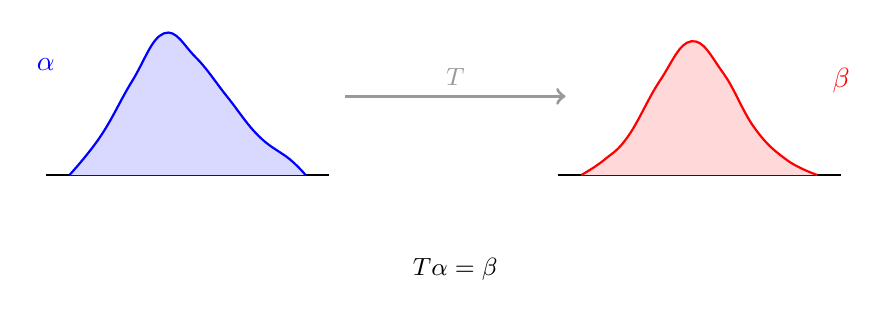
\begin{tikzpicture}[scale=1.0]
  % --- $\X$ と $\alpha$ ---
  \begin{scope}
    \draw[thick] (-0.3, 0) -- (3.3, 0);
    \node[below] at (1.5, -0.4) {$\X$};
    \fill[blue!15] plot[smooth, tension=0.7]
      coordinates {(0,0) (0.4,0.5) (0.8,1.2) (1.2,1.8) (1.6,1.5)
                   (2.0,1.0) (2.4,0.5) (2.8,0.2) (3.0,0)}
      -- cycle;
    \draw[thick, blue] plot[smooth, tension=0.7]
      coordinates {(0,0) (0.4,0.5) (0.8,1.2) (1.2,1.8) (1.6,1.5)
                   (2.0,1.0) (2.4,0.5) (2.8,0.2) (3.0,0)};
    \node[blue] at (-0.3, 1.4) {$\alpha$};
  \end{scope}

  % --- 写像 T ---
  \draw[->, very thick, gray!80] (3.5, 1.0) -- (6.3, 1.0)
    node[midway, above, font=\small] {$T$};

  % --- $\Y$ と $\beta$ ---
  \begin{scope}[xshift=6.5cm]
    \draw[thick] (-0.3, 0) -- (3.3, 0);
    \node[below] at (1.5, -0.4) {$\Y$};
    \fill[red!15] plot[smooth, tension=0.7]
      coordinates {(0,0) (0.3,0.2) (0.6,0.5) (1.0,1.2) (1.4,1.7)
                   (1.8,1.3) (2.2,0.6) (2.6,0.2) (3.0,0)}
      -- cycle;
    \draw[thick, red] plot[smooth, tension=0.7]
      coordinates {(0,0) (0.3,0.2) (0.6,0.5) (1.0,1.2) (1.4,1.7)
                   (1.8,1.3) (2.2,0.6) (2.6,0.2) (3.0,0)};
    \node[red] at (3.3, 1.2) {$\beta$};
  \end{scope}

  % --- 押し出し条件 ---
  \node[font=\small] at (4.9, -1.2)
    {$T\pushforward \alpha = \beta$};
\end{tikzpicture}
\caption{Monge 問題．$\X$ 上の分布 $\alpha$ が写像 $T$ で $\Y$ 上の分布 $\beta$ に押し出される．押し出しの詳細は命題~\ref{prop:sem-dirac-pushforward} 付近の略図を参照．}
\label{fig:sem-monge}
\end{figure}

\subsection{Monge 問題の本質的困難}

\subsubsection{困難1：実行可能集合の非凸性}

$\X = \Y = \R$ とする．
このとき可測写像 $T \colon \R \to \R$ の全体は，点ごとの和・スカラー倍
$(tT_1 + (1-t)T_2)(x) \defeq t\, T_1(x) + (1-t)\, T_2(x)$
によりベクトル空間をなす．この空間の部分集合としての
Monge 問題の実行可能集合
\[
  \mathcal{T}(\alpha, \beta)
  \defeq \left\{ T \colon \X \to \Y \;\middle|\;
  T \text{ は可測},\; T\pushforward \alpha = \beta \right\}
\]
は一般に\textbf{凸でない}．

\begin{example}{実行可能集合の非凸性}{sem-nonconvex}
  $\alpha = \beta = \tfrac{1}{2}\delta_{-1} + \tfrac{1}{2}\delta_1$ とし，
  \[
    T_1(x) = x,\qquad T_2(x) = -x,\qquad t = \tfrac{1}{2}
  \]
  をとる．$\alpha$ の定義を代入し，命題~\ref{prop:sem-dirac-pushforward} (ii) を適用すると
  \begin{align*}
    {T_1}\pushforward \alpha
    &= {T_1}\pushforward \bigl(\tfrac{1}{2}\delta_{-1} + \tfrac{1}{2}\delta_{1}\bigr)
      && \text{（$\alpha$ の定義）} \\
    &= \tfrac{1}{2}\delta_{T_1(-1)} + \tfrac{1}{2}\delta_{T_1(1)}
      && \text{（命題~\ref{prop:sem-dirac-pushforward} (ii)）} \\
    &= \tfrac{1}{2}\delta_{-1} + \tfrac{1}{2}\delta_{1} = \beta
      && \text{（$T_1(x) = x$ より）}.
  \end{align*}
  同様に
  \begin{align*}
    {T_2}\pushforward \alpha
    &= {T_2}\pushforward \bigl(\tfrac{1}{2}\delta_{-1} + \tfrac{1}{2}\delta_{1}\bigr)
      && \text{（$\alpha$ の定義）} \\
    &= \tfrac{1}{2}\delta_{T_2(-1)} + \tfrac{1}{2}\delta_{T_2(1)}
      && \text{（命題~\ref{prop:sem-dirac-pushforward} (ii)）} \\
    &= \tfrac{1}{2}\delta_{1} + \tfrac{1}{2}\delta_{-1} = \beta
      && \text{（$T_2(x) = -x$ より $T_2(-1) = 1,\, T_2(1) = -1$）}.
  \end{align*}
  よって $T_1, T_2 \in \mathcal{T}(\alpha, \beta)$ である．

  一方，$\bar{T} = \tfrac{1}{2}T_1 + \tfrac{1}{2}T_2$ は
  $\bar{T}(x) = \tfrac{1}{2}x + \tfrac{1}{2}(-x) = 0$
  すなわち $0$ を値にとる定値写像であり，
  $\bar{T}\pushforward\alpha = \delta_0 \neq \beta$．
  よって $\bar{T} \notin \mathcal{T}(\alpha, \beta)$ であり，
  $\mathcal{T}(\alpha, \beta)$ は凸でない．
\end{example}

\subsubsection{困難2：解の非存在}

\begin{example}{Monge 写像が存在しない場合}{sem-monge-noexist}
  $\alpha = \delta_0$（質量 $1$ が 1 点 $0$ に集中）と
  $\beta = \tfrac{1}{2}\delta_{-1} + \tfrac{1}{2}\delta_1$（2 点に質量 $\tfrac{1}{2}$ ずつ分散）
  を考える．任意の可測写像 $T \colon \R \to \R$ について
  命題~\ref{prop:sem-dirac-pushforward} (i) より
  \[
    T\pushforward \alpha = T\pushforward \delta_0 = \delta_{T(0)}
  \]
  となる．これは点 $T(0)$ に質量 $1$ を集中させた測度ゆえ
  $\delta_{T(0)}(\{T(0)\}) = 1$．一方 $\beta$ は任意の単点 $\{y\}$ に対し
  $\beta(\{y\}) \in \{0,\, \tfrac{1}{2}\}$（$y = \pm 1$ のとき $\tfrac{1}{2}$，
  それ以外で $0$）しか与えないので，どの $T(0) \in \R$ をとっても
  $\delta_{T(0)} \neq \beta$ である．
  したがって $T\pushforward \alpha = \beta$ をみたす $T$ は存在せず，
  $\mathcal{T}(\alpha, \beta) = \emptyset$（下図）．

  \begin{center}
  \begin{tikzpicture}[scale=1.0]
    \draw[->] (-1.8, 0) -- (1.8, 0);
    \draw[thick, blue] (0, 0) -- (0, 1.2);
    \fill[blue] (0, 1.2) circle (2pt);
    \node[below] at (0, -0.1) {$0$};
    \node[above, blue] at (0, 1.35) {$\alpha = \delta_0$};

    \draw[->, thick, dashed, gray] (2.2, 0.6) -- (3.2, 0.6);
    \node[above, gray] at (2.7, 0.6) {$T\, ?$};

    \begin{scope}[xshift=5cm]
      \draw[->] (-1.8, 0) -- (1.8, 0);
      \draw[thick, red] (-1, 0) -- (-1, 0.6);
      \fill[red] (-1, 0.6) circle (2pt);
      \draw[thick, red] (1, 0) -- (1, 0.6);
      \fill[red] (1, 0.6) circle (2pt);
      \node[below] at (-1, -0.1) {$-1$};
      \node[below] at (1, -0.1) {$1$};
      \node[above, red] at (0, 0.8) {$\beta = \tfrac{1}{2}\delta_{-1} + \tfrac{1}{2}\delta_1$};
    \end{scope}
  \end{tikzpicture}
  \end{center}
\end{example}

%% ============================================================
%% Kantorovich 問題
%% ============================================================
\section{Kantorovich 問題}
\label{sec:sem-kantorovich-problem}

\subsection{Kantorovich 緩和}
\label{sec:sem-kantorovich}

\subsubsection{問題の定義}

\begin{definition}{Kantorovich 問題}{sem-kantorovich}
  $\X, \Y$ 上の確率測度 $\alpha \in \Mm_+^1(\X)$, $\beta \in \Mm_+^1(\Y)$ と
  可測関数 $c \colon \X \times \Y \to \R_+$ に対して，
  \textbf{カップリング集合}
  \[
    \Couplings(\alpha, \beta) \defeq
    \left\{ \pi \in \Mm_+^1(\X \times \Y) \;\middle|\;
      \begin{aligned}
        &\pi(A \times \Y) = \alpha(A) \quad \forall\, A \in \Bb(\X), \\
        &\pi(\X \times B) = \beta(B)  \quad \forall\, B \in \Bb(\Y)
      \end{aligned}
    \right\}
  \]
  上で輸送コスト
  \[
    \MK_c(\alpha, \beta) \defeq
    \inf_{\pi \in \Couplings(\alpha, \beta)}
    \int_{\X \times \Y} c(x, y) \, \d\pi(x, y)
  \]
  を最小化する問題を\textbf{Kantorovich 問題}という．
\end{definition}

\begin{remark}{押し出しを用いたコンパクトな表現}{sem-marginal-pushforward}
  カップリング条件は，射影（定義~\ref{def:sem-projection}）
  $P_\X \colon (x,y) \mapsto x$，$P_\Y \colon (x,y) \mapsto y$ と
  押し出し（定義~\ref{def:sem-pushforward}）を用いると
  \[
    (P_\X)\pushforward \pi = \alpha, \qquad (P_\Y)\pushforward \pi = \beta
  \]
  とコンパクトに書ける．実際，任意の $A \in \Bb(\X)$ に対して
  \[
    \bigl((P_\X)\pushforward \pi\bigr)(A)
    = \pi\bigl(P_\X^{-1}(A)\bigr)
    = \pi\bigl(\{(x,y) \mid x \in A\}\bigr)
    = \pi(A \times \Y),
  \]
  ゆえに $(P_\X)\pushforward \pi = \alpha$ は
  $\pi(A \times \Y) = \alpha(A)$（$\forall\, A \in \Bb(\X)$）と同値である．
  $P_\Y$ についても同様．
\end{remark}

\begin{figure}[H]
\centering
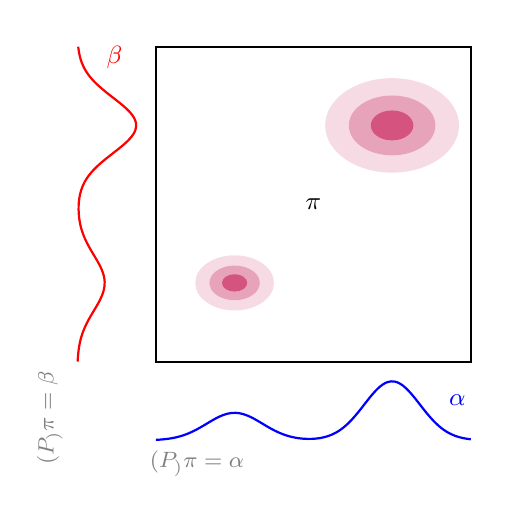
\begin{tikzpicture}[scale=1.0]
  % --- 正方形 X × Y ---
  \draw[thick] (0, 0) rectangle (4, 4);
  \node[font=\small, below right] at (4, 0) {$\X$};
  \node[font=\small, above left] at (0, 4) {$\Y$};

  % --- π を表す 2 つの集中領域（紫の濃淡，サイズで重みを表現）---
  % 小さい山: (1, 1) ; 大きい山: (3, 3)
  \fill[purple!20, opacity=0.7] (1.0, 1.0) ellipse (0.5 and 0.35);
  \fill[purple!45, opacity=0.7] (1.0, 1.0) ellipse (0.32 and 0.22);
  \fill[purple!75, opacity=0.8] (1.0, 1.0) ellipse (0.16 and 0.11);
  \fill[purple!20, opacity=0.7] (3.0, 3.0) ellipse (0.85 and 0.6);
  \fill[purple!45, opacity=0.7] (3.0, 3.0) ellipse (0.55 and 0.38);
  \fill[purple!75, opacity=0.8] (3.0, 3.0) ellipse (0.27 and 0.19);
  \node[font=\small] at (2.0, 2.0) {$\pi$};

  % --- α: X への射影（下方，2 山の密度曲線；高さ非対称） ---
  \draw[blue, thick, smooth, samples=80, domain=0:4]
    plot (\x, {-1 + 0.35*exp(-(\x-1.0)*(\x-1.0)*4)
                + 0.75*exp(-(\x-3.0)*(\x-3.0)*4)});
  \node[blue, font=\small, anchor=north west] at (3.6, -0.3) {$\alpha$};
  \node[font=\footnotesize, gray, anchor=west] at (-0.2, -1.3)
    {$(P_\X)\pushforward \pi = \alpha$};

  % --- β: Y への射影（左方，2 山の密度曲線；高さ非対称） ---
  \draw[red, thick, smooth, samples=80, domain=0:4, variable=\y]
    plot ({-1 + 0.35*exp(-(\y-1.0)*(\y-1.0)*4)
            + 0.75*exp(-(\y-3.0)*(\y-3.0)*4)}, \y);
  \node[red, font=\small, anchor=south east] at (-0.3, 3.6) {$\beta$};
  \node[font=\footnotesize, gray, anchor=base east, rotate=90] at (-1.3, 0.0)
    {$(P_\Y)\pushforward \pi = \beta$};
\end{tikzpicture}
\caption{カップリング $\pi \in \Couplings(\alpha, \beta)$ の概念図．
$\X \times \Y$ 上に分布する $\pi$（中央の紫領域）について，
$\X$ への射影が $\alpha$，$\Y$ への射影が $\beta$ に一致する．}
\label{fig:sem-coupling-continuous}
\end{figure}

\begin{figure}[htbp]
\centering
\begin{tikzpicture}[scale=0.95]
  % Monge (left)
  \node[above] at (1.5, 3.3) {\textbf{Monge 写像}};
  \fill[blue] (0.5, 2.5) circle (3pt) node[left] {\small $x_1$};
  \fill[blue] (0.5, 1.5) circle (3pt) node[left] {\small $x_2$};
  \fill[blue] (0.5, 0.5) circle (3pt) node[left] {\small $x_3$};
  \fill[red] (2.5, 2.5) circle (3pt) node[right] {\small $y_1$};
  \fill[red] (2.5, 1.5) circle (3pt) node[right] {\small $y_2$};
  \draw[->, thick] (0.7, 2.5) -- (2.3, 2.5);
  \draw[->, thick] (0.7, 1.5) -- (2.3, 2.5);
  \draw[->, thick] (0.7, 0.5) -- (2.3, 1.5);
  \node[below, text width=3cm, align=center] at (1.5, -0.2) {\small 各点は1つの\\行き先のみ};

  % Kantorovich (right)
  \begin{scope}[xshift=5.5cm]
    \node[above] at (1.5, 3.3) {\textbf{Kantorovich カップリング}};
    \fill[blue] (0.5, 2.5) circle (3pt) node[left] {\small $x_1$};
    \fill[blue] (0.5, 1.5) circle (3pt) node[left] {\small $x_2$};
    \fill[blue] (0.5, 0.5) circle (3pt) node[left] {\small $x_3$};
    \fill[red] (2.5, 2.5) circle (3pt) node[right] {\small $y_1$};
    \fill[red] (2.5, 1.5) circle (3pt) node[right] {\small $y_2$};
    \draw[->, thick] (0.7, 2.5) -- (2.3, 2.5);
    \draw[->, thick, blue!60] (0.7, 1.5) -- (2.3, 2.5);
    \draw[->, thick, red!60] (0.7, 1.5) -- (2.3, 1.5);
    \draw[->, thick] (0.7, 0.5) -- (2.3, 1.5);
    \node[right, font=\small] at (1.6, 1.8) {分割};
    \node[below, text width=3cm, align=center] at (1.5, -0.2) {\small 質量の分割を\\許す};
  \end{scope}
\end{tikzpicture}
\caption{Monge 写像と Kantorovich カップリングの対比．Monge 写像は各点を1つの行き先に送るが，Kantorovich カップリングは質量の分割を許す．}
\label{fig:sem-monge-vs-kantorovich}
\end{figure}

\subsubsection{離散化}

$\mathbf{a} \in \R_{++}^n$（$\sum_i a_i = 1$），$\mathbf{b} \in \R_{++}^m$（$\sum_j b_j = 1$），
$x_1, \ldots, x_n \in \X$，$y_1, \ldots, y_m \in \Y$ および
可測関数 $c \colon \X \times \Y \to \R_+$ を所与とし，
\begin{align*}
  \alpha \defeq \sum_{i=1}^n a_i\, \delta_{x_i} \in \Mm_+^1(\X), \qquad
  \beta  \defeq \sum_{j=1}^m b_j\, \delta_{y_j} \in \Mm_+^1(\Y)
\end{align*}
とおく．$\alpha, \beta$ を Kantorovich 問題（定義~\ref{def:sem-kantorovich}）に代入すると，
次の命題が示すとおり連続問題は自然に行列最適化へ帰着する．

\begin{proposition}{連続 Kantorovich 問題の離散化}{sem-discrete-kantorovich}
  行列 $\mathbf{C} \defeq \bigl(c(x_i, y_j)\bigr)_{i,j} \in \R_+^{n \times m}$ および
  \textbf{離散カップリング集合}
  \[
    \CouplingsD(\mathbf{a}, \mathbf{b}) \defeq
    \left\{ \mathbf{P} \in \R_+^{n \times m} \;\middle|\;
      \mathbf{P}\ones_m = \mathbf{a},\;
      \mathbf{P}^\top\ones_n = \mathbf{b}
    \right\}
  \]
  に対して
  \[
    \MK_c(\alpha, \beta)
    = \min_{\mathbf{P} \in \CouplingsD(\mathbf{a}, \mathbf{b})}
      \inner{\mathbf{C}}{\mathbf{P}}
  \]
  が成り立つ．ここで $\inner{\mathbf{C}}{\mathbf{P}} \defeq \sum_{i,j} C_{i,j} P_{i,j}$ はフロベニウス内積
  （定義~\ref{def:sem-frobenius-inner}）である．
\end{proposition}
\begin{proof}
  次の 2 点を示す：
  \begin{itemize}
    \item[(A)] コスト保存全単射
      $\varphi \colon \Couplings(\alpha,\beta) \xrightarrow{\sim} \CouplingsD(\mathbf{a},\mathbf{b})$
      が存在する．
    \item[(B)] $\varphi$ はコストを保存する：
      $\displaystyle\int_{\X\times\Y} c\,\d\pi = \inner{\mathbf{C}}{\varphi(\pi)}$．
  \end{itemize}
  (A)(B) が示されれば，$\Couplings(\alpha,\beta)$ 上の inf と
  $\CouplingsD(\mathbf{a},\mathbf{b})$ 上の inf が一致し，
  後者は後続の主張~\ref{clm:sem-discrete-kantorovich-existence} のコンパクト性から
  最小値として達成される．

  \medskip
  \textbf{(A-1) $\varphi$ の構成（カップリングの台）．}
  任意の $\pi \in \Couplings(\alpha, \beta)$ をとる．
  周辺条件 $\pi(A \times \Y) = \alpha(A)$（$\forall A \in \Bb(\X)$）と
  $\alpha(\X \setminus \{x_1,\ldots,x_n\}) = 0$ から
  \[
    \pi\bigl((\X \setminus \{x_1,\ldots,x_n\}) \times \Y\bigr) = 0,
  \]
  同様に $\pi(\X \times (\Y \setminus \{y_1,\ldots,y_m\})) = 0$．
  よって $\pi$ は有限格子 $\{x_1,\ldots,x_n\} \times \{y_1,\ldots,y_m\}$ 上のみに質量を持ち，
  \[
    \varphi(\pi)_{i,j} \defeq P_{i,j} \defeq \pi\bigl(\{(x_i, y_j)\}\bigr) \geq 0
  \]
  と定めると $\pi = \sum_{i,j} P_{i,j}\, \delta_{(x_i, y_j)}$ と書ける．

  \medskip
  \textbf{(A-2) $\varphi(\pi) \in \CouplingsD(\mathbf{a},\mathbf{b})$（周辺条件 $\leftrightarrow$ 行・列和条件）．}
  周辺条件 $\pi(\{x_k\} \times \Y) = \alpha(\{x_k\}) = a_k$ から
  \[
    \sum_{j=1}^m P_{k,j} = a_k \quad (\forall k),
    \qquad\text{すなわち}\quad
    \mathbf{P}\ones_m = \mathbf{a}.
  \]
  同様に $\pi(\X \times \{y_l\}) = \beta(\{y_l\}) = b_l$ から
  $\mathbf{P}^\top\ones_n = \mathbf{b}$．
  ゆえに $\mathbf{P} \in \CouplingsD(\mathbf{a},\mathbf{b})$．

  \medskip
  \textbf{(A-3) $\varphi$ は全単射．}
  \textit{全射}：任意の $\mathbf{P} \in \CouplingsD(\mathbf{a},\mathbf{b})$ に対し
  $\pi' \defeq \sum_{i,j} P_{i,j}\,\delta_{(x_i,y_j)}$ とおくと，
  任意の $A \in \Bb(\X)$ について
  \[
    \pi'(A \times \Y)
    = \sum_{i:\,x_i \in A} \sum_j P_{i,j}
    = \sum_{i:\,x_i \in A} a_i
    = \alpha(A),
  \]
  同様に $\pi'(\X \times B) = \beta(B)$（$\forall B \in \Bb(\Y)$）だから
  $\pi' \in \Couplings(\alpha,\beta)$，かつ $\varphi(\pi') = \mathbf{P}$．
  \textit{単射}：$\varphi(\pi_1) = \varphi(\pi_2) = \mathbf{P}$ とすれば，
  (A-1) より $\pi_1 = \pi_2 = \sum_{i,j} P_{i,j}\,\delta_{(x_i,y_j)}$．

  \medskip
  \textbf{(B) $\varphi$ はコストを保存する．}
  測度に関する積分の線形性（命題~\ref{prop:sem-measure-linearity}）と
  Dirac 測度に対する積分（主張~\ref{clm:sem-dirac-integral}）から
  \[
    \int_{\X \times \Y} c(x, y)\, \d\pi(x, y)
    = \sum_{i,j} P_{i,j}\, c(x_i, y_j)
    = \inner{\mathbf{C}}{\mathbf{P}}.
  \]

  \medskip
  \textbf{結論．}
  (A)(B) より $\varphi$ はコストを保存する全単射だから，
  \[
    \MK_c(\alpha, \beta)
    = \inf_{\pi \in \Couplings(\alpha, \beta)}
      \int_{\X \times \Y} c\, \d\pi
    = \inf_{\mathbf{P} \in \CouplingsD(\mathbf{a}, \mathbf{b})}
      \inner{\mathbf{C}}{\mathbf{P}}.
  \]
  右辺の inf は $\CouplingsD(\mathbf{a},\mathbf{b})$ のコンパクト性
  （主張~\ref{clm:sem-discrete-kantorovich-existence}）により達成されるから
  $\inf = \min$ が成り立つ．
\end{proof}

右辺の最適値を
\[
  \MKD_{\mathbf{C}}(\mathbf{a}, \mathbf{b})
  \defeq \min_{\mathbf{P} \in \CouplingsD(\mathbf{a}, \mathbf{b})} \inner{\mathbf{C}}{\mathbf{P}}
\]
と書き，\textbf{離散 Kantorovich 問題}と呼ぶ．

\begin{example}{工場からスーパーへの輸送}{sem-factory-supermarket}
  2 つの工場 $x_1, x_2$ から 2 つのスーパー $y_1, y_2$ へ商品を輸送する状況を考える．
  各工場の供給割合を $\mathbf{a} = (2/3,\; 1/3)^\top$，
  各スーパーの需要割合を $\mathbf{b} = (1/3,\; 2/3)^\top$ とし，
  輸送コスト行列を
  \[
    \mathbf{C} =
    \begin{pmatrix}
      C_{1,1} & C_{1,2} \\
      C_{2,1} & C_{2,2}
    \end{pmatrix}
    =
    \begin{pmatrix}
      1 & 2 \\
      3 & 1
    \end{pmatrix}
  \]
  とする（図~\ref{fig:sem-factory-supermarket-cost}）．

  \begin{figure}[H]
    \centering
    \begin{tikzpicture}[
      factory/.style={draw, fill=blue!15, rounded corners, minimum width=1.6cm, minimum height=0.9cm},
      super/.style={draw, fill=orange!15, rounded corners, minimum width=1.6cm, minimum height=0.9cm},
      every edge/.style={draw, -{Stealth[length=5pt]}, thick},
      cost label/.style={font=\small, fill=white, inner sep=1.5pt},
    ]
      % 工場ノード
      \node[factory] (x1) at (0, 1.5) {$x_1$};
      \node[factory] (x2) at (0, -1.5) {$x_2$};
      % スーパーノード
      \node[super] (y1) at (5, 1.5) {$y_1$};
      \node[super] (y2) at (5, -1.5) {$y_2$};
      % 供給・需要ラベル
      \node[left=0.3cm of x1, font=\small] {$a_1 = \tfrac{2}{3}$};
      \node[left=0.3cm of x2, font=\small] {$a_2 = \tfrac{1}{3}$};
      \node[right=0.3cm of y1, font=\small] {$b_1 = \tfrac{1}{3}$};
      \node[right=0.3cm of y2, font=\small] {$b_2 = \tfrac{2}{3}$};
      % コスト辺
      \draw (x1) edge node[cost label, pos=0.5, above] {$C_{1,1}=1$} (y1);
      \draw (x1) edge node[cost label, pos=0.35, below] {$C_{1,2}=2$} (y2);
      \draw (x2) edge node[cost label, pos=0.35, above] {$C_{2,1}=3$} (y1);
      \draw (x2) edge node[cost label, pos=0.5, below] {$C_{2,2}=1$} (y2);
      % ラベル
      \node[above=0.3cm of x1, font=\small\bfseries] {工場};
      \node[above=0.3cm of y1, font=\small\bfseries] {スーパー};
    \end{tikzpicture}
    \caption{輸送コストのネットワーク．各辺の数値は単位量あたりの輸送コスト $C_{i,j}$ を表す．}
    \label{fig:sem-factory-supermarket-cost}
  \end{figure}

  コストの安い経路 $x_1 \to y_1$（コスト $1$）と $x_2 \to y_2$（コスト $1$）を
  最大限利用し，残りを $x_1 \to y_2$（コスト $2$）で補うのが最適であり，
  \[
    \mathbf{P}^{\star} =
    \begin{pmatrix}
      1/3 & 1/3 \\
      0 & 1/3
    \end{pmatrix}.
  \]

  $\mathbf{P}^{\star} \in \CouplingsD(\mathbf{a}, \mathbf{b})$ であることを周辺条件から確認する：
  \[
    \mathbf{P}^{\star}\ones_2
    = \begin{pmatrix} \tfrac{1}{3} + \tfrac{1}{3} \\ 0 + \tfrac{1}{3} \end{pmatrix}
    = \begin{pmatrix} \tfrac{2}{3} \\ \tfrac{1}{3} \end{pmatrix}
    = \mathbf{a},
    \qquad
    (\mathbf{P}^{\star})^\top\ones_2
    = \begin{pmatrix} \tfrac{1}{3} + 0 \\ \tfrac{1}{3} + \tfrac{1}{3} \end{pmatrix}
    = \begin{pmatrix} \tfrac{1}{3} \\ \tfrac{2}{3} \end{pmatrix}
    = \mathbf{b}.
  \]


  最適コストは
  \[
    \MKD_{\mathbf{C}}(\mathbf{a}, \mathbf{b})
    = \inner{\mathbf{C}}{\mathbf{P}^{\star}}
    = \sum_{i,j} C_{i,j} P_{i,j}^{\star}
    = 1 \cdot \tfrac{1}{3} + 2 \cdot \tfrac{1}{3} + 3 \cdot 0 + 1 \cdot \tfrac{1}{3}
    = \tfrac{4}{3}.
  \]

  \begin{figure}[H]
    \centering
    \begin{tikzpicture}[
      factory/.style={draw, fill=blue!15, rounded corners, minimum width=1.6cm, minimum height=0.9cm},
      super/.style={draw, fill=orange!15, rounded corners, minimum width=1.6cm, minimum height=0.9cm},
      every edge/.style={draw, -{Stealth[length=5pt]}},
      cost label/.style={font=\small, fill=white, inner sep=1.5pt},
    ]
      % 工場ノード
      \node[factory] (x1) at (0, 1.5) {$x_1$};
      \node[factory] (x2) at (0, -1.5) {$x_2$};
      % スーパーノード
      \node[super] (y1) at (5, 1.5) {$y_1$};
      \node[super] (y2) at (5, -1.5) {$y_2$};
      % 供給・需要ラベル
      \node[left=0.3cm of x1, font=\small] {$a_1 = \tfrac{2}{3}$};
      \node[left=0.3cm of x2, font=\small] {$a_2 = \tfrac{1}{3}$};
      \node[right=0.3cm of y1, font=\small] {$b_1 = \tfrac{1}{3}$};
      \node[right=0.3cm of y2, font=\small] {$b_2 = \tfrac{2}{3}$};
      % 最適輸送の辺（太さで量を表現，コスト併記）
      \draw[line width=2.0pt, blue!70] (x1) edge node[cost label, above] {$P_{1,1}^{\star}=\tfrac{1}{3}$\;\scriptsize$(C=1)$} (y1);
      \draw[line width=2.0pt, blue!70] (x1) edge node[cost label, pos=0.35, below] {$P_{1,2}^{\star}=\tfrac{1}{3}$\;\scriptsize$(C=2)$} (y2);
      \draw[line width=0.4pt, gray, dashed] (x2) edge node[cost label, pos=0.35, above, text=gray] {$P_{2,1}^{\star}=0$\;\scriptsize$(C=3)$} (y1);
      \draw[line width=2.0pt, blue!70] (x2) edge node[cost label, below] {$P_{2,2}^{\star}=\tfrac{1}{3}$\;\scriptsize$(C=1)$} (y2);
      % ラベル
      \node[above=0.3cm of x1, font=\small\bfseries] {工場};
      \node[above=0.3cm of y1, font=\small\bfseries] {スーパー};
    \end{tikzpicture}
    \caption{最適輸送計画 $\mathbf{P}^{\star}$．
    安価な経路 $x_1 \to y_1$（コスト $1$）と $x_2 \to y_2$（コスト $1$）を
    最大限利用し，残りを $x_1 \to y_2$（コスト $2$）で補う．
    高コストの $x_2 \to y_1$（コスト $3$）は使われない．}
    \label{fig:sem-factory-supermarket-opt}
  \end{figure}
\end{example}


\begin{figure}[H]
\centering
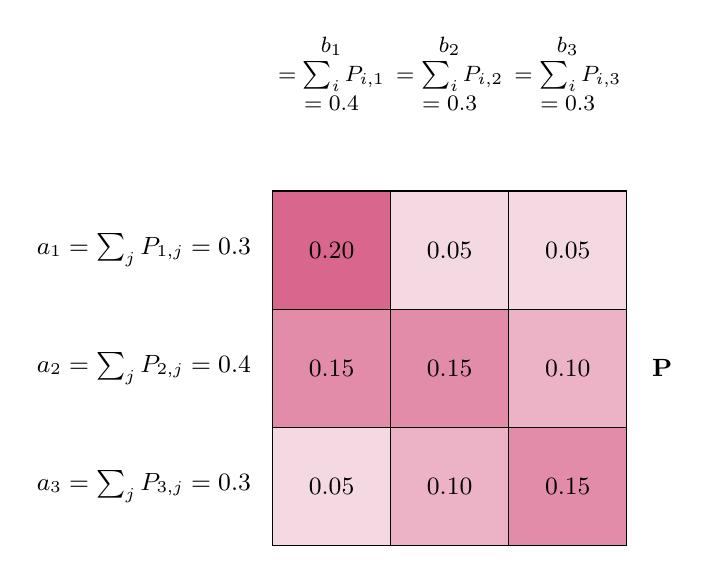
\begin{tikzpicture}[scale=1.0]
  % ---- 上ヘッダー: b_j = sum_i P_{i,j} = value（3 行に折りたたみ） ----
  \node[font=\footnotesize, anchor=south, align=center] at (1.5, 0.15)
    {$b_1$ \\[1pt] $= \textstyle\sum_i P_{i,1}$ \\[1pt] $= 0.4$};
  \node[font=\footnotesize, anchor=south, align=center] at (3.0, 0.15)
    {$b_2$ \\[1pt] $= \textstyle\sum_i P_{i,2}$ \\[1pt] $= 0.3$};
  \node[font=\footnotesize, anchor=south, align=center] at (4.5, 0.15)
    {$b_3$ \\[1pt] $= \textstyle\sum_i P_{i,3}$ \\[1pt] $= 0.3$};

  % ---- 左ヘッダー: a_i = sum_j P_{i,j} = value（1 行） ----
  \node[font=\small, anchor=east] at (0.6, -1.5) {$a_1 = \sum_j P_{1,j} = 0.3$};
  \node[font=\small, anchor=east] at (0.6, -3.0) {$a_2 = \sum_j P_{2,j} = 0.4$};
  \node[font=\small, anchor=east] at (0.6, -4.5) {$a_3 = \sum_j P_{3,j} = 0.3$};

  % ---- 行列 P （3x3） ----
  \foreach \i/\j/\v/\op in {%
    1/1/0.20/60, 1/2/0.05/15, 1/3/0.05/15,%
    2/1/0.15/45, 2/2/0.15/45, 2/3/0.10/30,%
    3/1/0.05/15, 3/2/0.10/30, 3/3/0.15/45}{%
    \fill[purple!\op] (1.5*\j - 0.75, -1.5*\i + 0.75)
                      rectangle (1.5*\j + 0.75, -1.5*\i - 0.75);
    \draw (1.5*\j - 0.75, -1.5*\i + 0.75)
          rectangle (1.5*\j + 0.75, -1.5*\i - 0.75);
    \node[font=\small] at (1.5*\j, -1.5*\i) {$\v$};
  }

  % ---- P ラベル ----
  \node[font=\small\bfseries] at (5.7, -3.0) {$\mathbf{P}$};
\end{tikzpicture}
\caption{離散カップリング $\mathbf{P} \in \CouplingsD(\mathbf{a}, \mathbf{b})$ の構造．
中央の $3 \times 3$ 行列が $\mathbf{P}$（色の濃さが値 $P_{i,j}$ の大きさを表す）．}
\label{fig:sem-coupling-matrix}
\end{figure}

\subsubsection{最適解の存在と性質}

\begin{claim}{離散 Kantorovich 問題の解の存在}{sem-discrete-kantorovich-existence}
  任意の $\mathbf{a} \in \R_{++}^n$，$\mathbf{b} \in \R_{++}^m$
  （$\sum_i a_i = \sum_j b_j = 1$）と $\mathbf{C} \in \R_+^{n \times m}$ に対して，
  \[
    \MKD_{\mathbf{C}}(\mathbf{a}, \mathbf{b}) = \inner{\mathbf{C}}{\mathbf{P}^*}
  \]
  をみたす $\mathbf{P}^* \in \CouplingsD(\mathbf{a}, \mathbf{b})$ が存在する．
\end{claim}

\begin{proof}
  以下の3点を示せばよい：
  (i) $\CouplingsD(\mathbf{a}, \mathbf{b}) \neq \emptyset$，
  (ii) $\CouplingsD(\mathbf{a}, \mathbf{b}) \subset \R^{n \times m}$ はコンパクト，
  (iii) 目的関数 $\mathbf{P} \mapsto \inner{\mathbf{C}}{\mathbf{P}}$ は連続．

  \textbf{(i) 非空性．}
  $\mathbf{P}_0 \defeq \mathbf{a}\mathbf{b}^\top$ を考える．
  これは各成分が $(P_0)_{i,j} = a_i b_j$ で定まる $n \times m$ 行列であり，
  $a_i, b_j > 0$ より $\mathbf{P}_0 \geq \mathbf{0}$ である．
  行和について，$\sum_j b_j = 1$ を用いて
  \[
    (\mathbf{P}_0 \ones_m)_i
    = \sum_{j=1}^m a_i b_j
    = a_i \sum_{j=1}^m b_j
    = a_i,
  \]
  すなわち $\mathbf{P}_0 \ones_m = \mathbf{a}$．
  同様に $\sum_i a_i = 1$ から $\mathbf{P}_0^\top \ones_n = \mathbf{b}$．
  よって $\mathbf{P}_0 \in \CouplingsD(\mathbf{a}, \mathbf{b})$．
  （$\mathbf{P}_0$ は連続版における独立カップリング $\alpha \otimes \beta$
  の離散版に相当する．）

  \textbf{(ii) コンパクト性．}
  $\CouplingsD(\mathbf{a}, \mathbf{b})$ の定義条件
  $\mathbf{P}\ones_m = \mathbf{a}$，$\mathbf{P}^\top \ones_n = \mathbf{b}$，$\mathbf{P} \geq \mathbf{0}$
  はいずれも各成分 $P_{i,j}$ の連続関数による等式・不等式であるから，
  $\CouplingsD(\mathbf{a}, \mathbf{b})$ は $\R^{n \times m}$ の閉集合である．
  さらに，行和条件 $\sum_j P_{i,j} = a_i$ と $P_{i,j} \geq 0$ から
  $0 \leq P_{i,j} \leq a_i \leq 1$ が従い有界．
  $\R^{n \times m}$ における有界閉集合はコンパクト
  （定理~\ref{thm:sem-heine-borel}）．

  \textbf{(iii) 連続性．}
  各 $P_{i,j} \colon \R^{n \times m} \to \R$ は座標射影であるから連続であり，
  定数 $C_{i,j}$ との積 $C_{i,j} P_{i,j}$ も連続である．
  よって $\mathbf{P} \mapsto \inner{\mathbf{C}}{\mathbf{P}} = \sum_{i,j} C_{i,j} P_{i,j}$
  は連続関数の有限和として連続．

  以上 (i)--(iii) と Weierstrass の最大値の定理
  （定理~\ref{thm:sem-weierstrass}）より，
  空でないコンパクト集合上の連続関数は最小値を達成する．
  したがって最適解 $\mathbf{P}^*$ が存在する．
\end{proof}

\begin{claim}{最適解集合は凸かつコンパクト}{sem-optimal-face}
  最適解の集合
  \[
    S^*
    \defeq
    \bigl\{ \mathbf{P}^* \in \CouplingsD(\mathbf{a}, \mathbf{b})
    \bigm|
    \inner{\mathbf{C}}{\mathbf{P}^*} = \MKD_{\mathbf{C}}(\mathbf{a}, \mathbf{b})
    \bigr\}
  \]
  は凸かつコンパクトである．
\end{claim}

\begin{proof}
  \textbf{凸性．}
  $\mathbf{P}^*, \mathbf{Q}^* \in S^*$ と $t \in [0,1]$ に対し，
  $\mathbf{R} \defeq t\mathbf{P}^* + (1-t)\mathbf{Q}^*$ は
  $\CouplingsD(\mathbf{a}, \mathbf{b})$ の凸性から
  $\CouplingsD(\mathbf{a}, \mathbf{b})$ に属し，
  \[
    \inner{\mathbf{C}}{\mathbf{R}}
    = t\inner{\mathbf{C}}{\mathbf{P}^*} + (1-t)\inner{\mathbf{C}}{\mathbf{Q}^*}
    = \MKD_{\mathbf{C}}(\mathbf{a}, \mathbf{b}).
  \]

  \textbf{コンパクト性．}
  $S^*
  = \CouplingsD(\mathbf{a}, \mathbf{b})
  \cap \{\mathbf{P} \mid \inner{\mathbf{C}}{\mathbf{P}}
  = \MKD_{\mathbf{C}}(\mathbf{a}, \mathbf{b})\}$
  はコンパクト集合と閉集合の共通部分．
\end{proof}

\begin{example}{最適解の非一意性}{sem-nonunique-example}
  $n = m = 2$，$\mathbf{a} = \mathbf{b} = (1/2,\; 1/2)$ とし，
  コスト行列を
  \[
    \mathbf{C} = \begin{pmatrix} 1 & 3 \\ 3 & 5 \end{pmatrix}
  \]
  とする（$C_{11} + C_{22} = 6 = C_{12} + C_{21}$）．
  周辺条件の連立を解くと自由変数は $P_{1,1} \in [0,1/2]$ の1つで，
  残りは $P_{1,2} = P_{2,1} = 1/2 - P_{1,1}$，$P_{2,2} = P_{1,1}$ と定まる．
  $s \defeq 1 - 2P_{1,1} \in [0,1]$ とおけば $\mathbf{P} = (1-s)\mathbf{P}_1 + s\mathbf{P}_2$ となり，
  $\CouplingsD(\mathbf{a}, \mathbf{b})$ は
  \[
    \mathbf{P}_1
    = \begin{pmatrix} 1/2 & 0 \\ 0 & 1/2 \end{pmatrix},
    \qquad
    \mathbf{P}_2
    = \begin{pmatrix} 0 & 1/2 \\ 1/2 & 0 \end{pmatrix}
  \]
  を端点とする線分である．両者のコストはともに
  \[
    \inner{\mathbf{C}}{\mathbf{P}_1}
    = \tfrac{1}{2} + \tfrac{5}{2} = 3,
    \qquad
    \inner{\mathbf{C}}{\mathbf{P}_2}
    = \tfrac{3}{2} + \tfrac{3}{2} = 3
  \]
  で等しい．
  したがって任意の $t \in [0, 1]$ に対して
  $t\mathbf{P}_1 + (1-t)\mathbf{P}_2$ が最適であり，
  $S^* = \CouplingsD(\mathbf{a}, \mathbf{b})$ となる．

  この非一意性は
  $C_{11} + C_{22} = C_{12} + C_{21}$ から生じる．
  逆に $C_{11} + C_{22} \neq C_{12} + C_{21}$ ならば
  2頂点のコストが異なるため最適解は一意となる．
\end{example}

\begin{remark}{エントロピー正則化による一意性の回復}{sem-entropy-uniqueness-preview}
  離散 Kantorovich 問題の最適解は一般に一意でないが，
  \textbf{離散エントロピー}
  \[
    \Hb(\mathbf{P}) \defeq -\sum_{i,j} P_{i,j}(\log P_{i,j} - 1)
  \]
  （定義~\ref{def:sem-discrete-entropy}）を用いた正則化パラメータ $\varepsilon > 0$
  によるエントロピー正則化
  \[
    \min_{\mathbf{P} \in \CouplingsD(\mathbf{a}, \mathbf{b})}
    \left\{
      \inner{\mathbf{C}}{\mathbf{P}}
      - \varepsilon \Hb(\mathbf{P})
    \right\}
  \]
  は狭義凸最適化であり，最適解は一意に定まる（第~\ref{ch:seminar-03-entropic}章）．
\end{remark}

